\chapter{Evaluation}
\label{chapter6}
Um die Praxistauglichkeit zu überprüfen, werden nun ausgewählte Daten
mithilfe des entwickelten Tools geclustert.
Die Ergebnisse werden bewertet.
Zur Bewertung des Clusterings unterscheidet man \emph{externe}
und \emph{interne} Indizes \citep{aghabozorgi_time-series_2015, warren_liao_clustering_2005}.
Bei einem \emph{externen Index} werden \emph{Ground-Truth-Daten} extern bereitgestellt.
Nach dem Clustering kann der Grad der Übereinstimmung zwischen gefundenen Cluster
und den vorgegebenen Clustern überprüft werden.
In diesem Kapitel werden die Daten mithilfe der Visualisierung manuell geclustert.
In \autoref{6-GroundTruth} werden die gefundenen Cluster mit den erwarteten verglichen.
Bei \emph{internen Indizes} muss die Qualität der Cluster hingegen
ohne zusätzliche Informationen überprüft werden \citep{aghabozorgi_time-series_2015, warren_liao_clustering_2005}.
Dazu sollen in \autoref{6-Statistical} \emph{desktiptive Statistiken} genutzt werden.
Die Standardabweichung, der Mittelwert, das Maximum und das Minimum liefern
ein Maß für die Ähnlichkeit von Cluster-Komponenten.
Damit wird überprüft,
ob zusammengefasste Records tatsächlich einen hohen Grad an Übereinstimmung aufweisen.

\section{Einführende Bemerkungen}
\label{6-Bemerkungen}
Statt den gesamten in \autoref{2-StrukturDatensatz} beschriebenen Datensatz zu verwenden
sollen geeignete Teilmengen genutzt werden.
Zudem wurden die Daten zur Evaluation gefiltert bereitgestellt.
Zu kurze oder fehlerhafte Records wurden aussortiert.
Außerdem erfolgte eine Sortierung nach Personenzahl.
Das Filtern der Daten gehört nicht zu den Anforderungen an das entwickelte Tool
und wird daher nicht in dieser Arbeit betrachtet.
Dennoch sollte dem Nutzer bewusst sein,
dass mit gefilterten Daten gegebenfalls aussagekräftigere Ergebnisse erzielbar sind.
Gerade die separate Betrachtung von Records unterschiedlicher Personenzahl kann helfen,
wiederkehrende Bewegungsmuster durch Clustering zu erkennen.
Die Anzahl gibt dabei immer an wie viele Personen sich maximal
zu einem Zeitpunkt in der Aufnahme befinden.
In der Evaluation werden nur Records mit ein bis drei Personen betrachtet.

Ebenfalls zu erwähnen ist die Bedeutung eines geeigneten Threshold-Wertes für ein erfolgreiches Clustering.
Dieser kann je nach vorliegenden Daten, verwendeten Attributen und Zielstellung variieren.
Häufig ist daher ein {\glqq Herantasten\grqq} nötig.
In den später beschriebenen Szenarien war beispielsweise auffällig,
dass der Threshold bei Records mit einer Person deutlich niedriger war,
als bei Records mit mehreren Personen.
Abhängig davon wie viele Cluster am Ende erwünscht sind
und wie stark die Cluster-Bestandteile voneinander abweichen dürfen,
muss ein anderer Wert gewählt werden.

Die Ground-Truth-Daten wurden manuell mithilfe der Visualisierung erstellt.
Zunächst werden drei Minimalbeispiele betrachtet.
Dafür wurden für die Fälle eine bis drei Personen jeweils beliebig 25 Records gewählt.
Diese wurden mithilfe des Visualizers und Kinect Studio visualisiert und manuell in Cluster eingeteilt.
\autoref{fig:Clusters} zeigt jeweils die Visualisierung eines Repräsentanten der Cluster.
\begin{figure}[ht]
    \begin{center}
    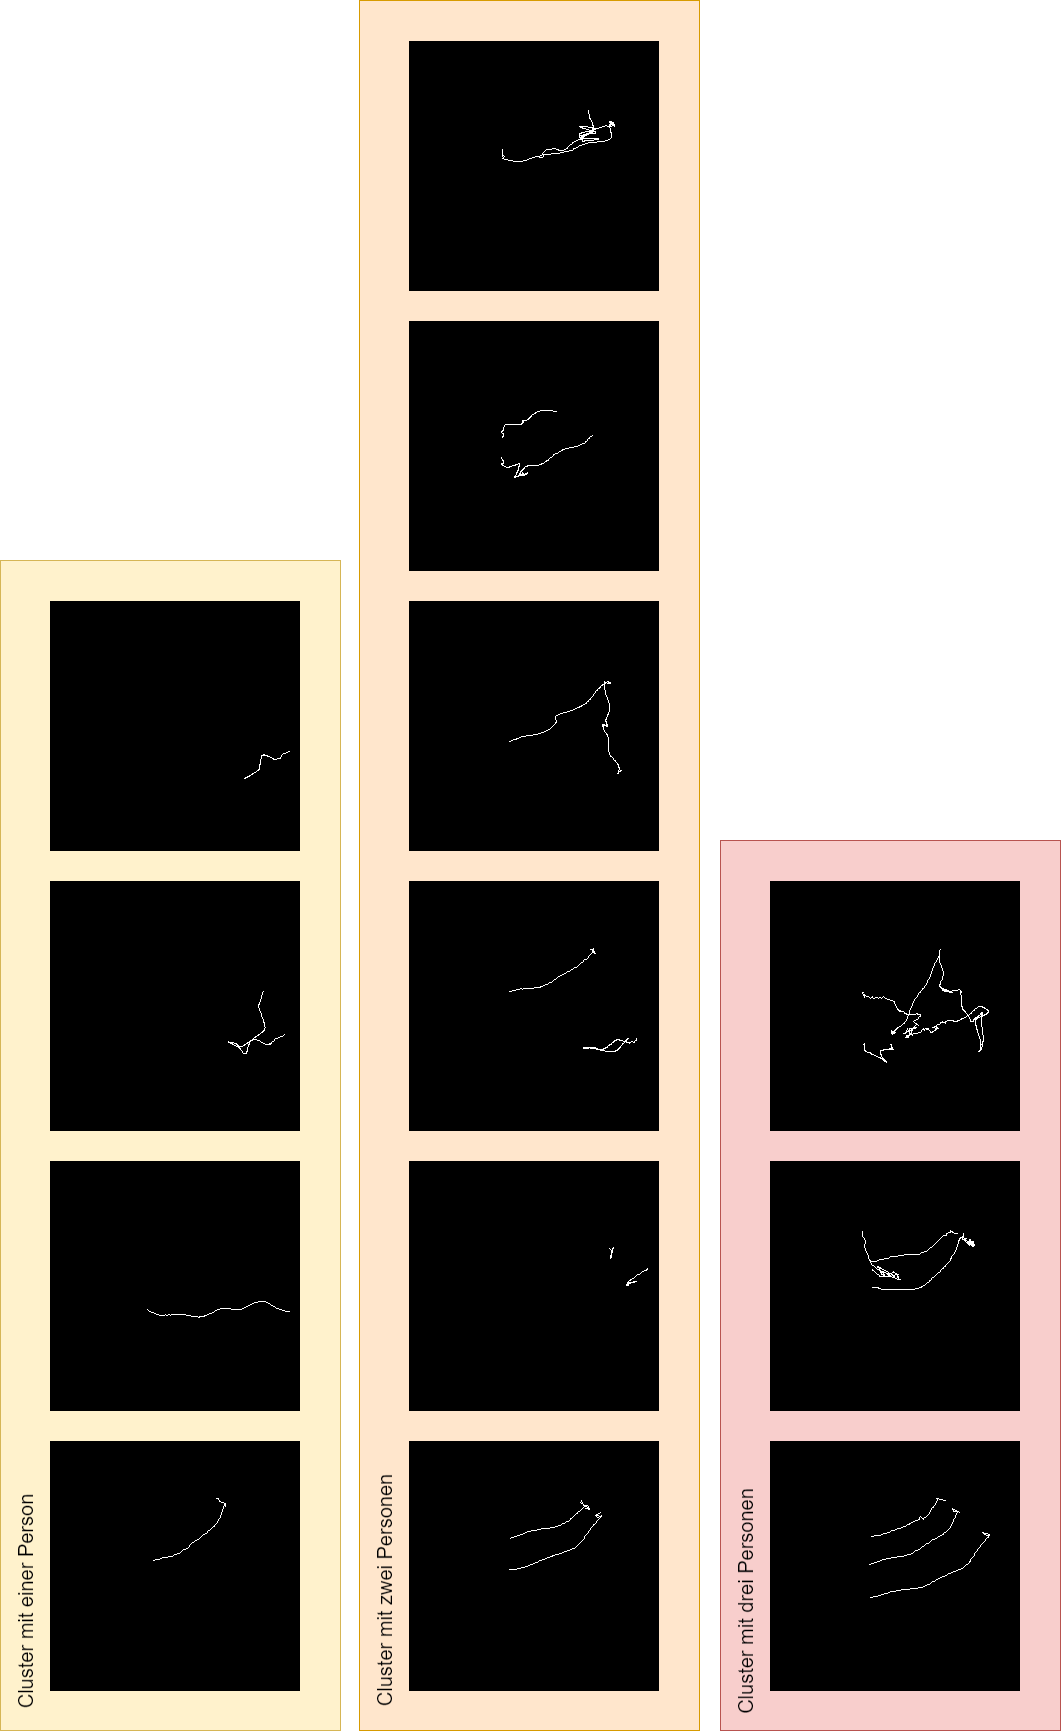
\includegraphics[width=0.8\textwidth]{clusters.png}
    \end{center}
    \caption{Repräsentanten der manuell erstellten Cluster.}
    \label{fig:Clusters}
\end{figure}
Die Ergebnisse und eine sprachliche Beschreibung des Inhalts
können im \emph{resources}-Verzeichnis des Projektordners eingesehen werden.
Das hierarchische Clustering wurde mit den x- und z-Werten als Vergleichsattribute gestartet.
Der Threshold wurde dabei jeweils so gewählt,
dass genau so viele Cluster entstehen wie auch manuell erkannt wurden.
Die Auswertung zeigt, dass die vom Tool berechneten Cluster genau mit den Ground-Truth Daten übereinstimmen.
Diese Minimalbeispiele sind aber nur bedingt aussagekräftig,
da lediglich eine kleine Teilmenge der tatsächlich vorhandenen Daten genutzt wird.
Manche Muster treten dadurch gegebenfalls überhaupt nicht auf.
In \autoref{6-GroundTruth} soll daher die Analyse auf alle vorhandenen gefilterten Daten
für ein bis drei Personen ausgeweitet werden.
Aufgrund der Vielzahl der Daten ist das manuelle Clustering allerdings nicht so
zuverlässig möglich wie in den oben beschriebenen Minimalbeispielen.
Die Daten wurden aber nach bestem Wissen auf die wichtigsten Bewegungen hin untersucht.
Spezielle Bewegungen die nur einmalig auftreten wurden ignoriert.
Ziel ist es zu überprüfen,
ob häufig wiederkehrende Muster vom Tool korrekt erkannt werden.

\section{Ground-Truth Analyse}
\label{6-GroundTruth}
Im gefilterten Datensatz mit drei Personen befinden sich insgesamt 103 Records.
Die manuelle Einteilung ergab,
dass es sich bei den meisten darin vorkommenden Bewegungsabläufen
um spezielle Bewegungen handelt, die nicht häufiger auftreten.
Sie sollen im Folgenden nicht aufgeführt werden.
Allerdings wurde ein eindeutiges Cluster identifiziert.
\autoref{fig:3PersClust1} zeigt einen Repräsentanten dieses Clustes.
\begin{figure}[ht]
    \begin{center}
    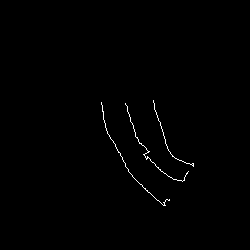
\includegraphics[width=0.2\textwidth]{representation3PersCluster1.png}
    \end{center}
    \caption{Repräsentant des nicht trivialen Clusters mit drei Personen.}
    \label{fig:3PersClust1}
\end{figure}
Es handelt sich dabei um drei Personen die nebeneinander durch den Sensorbereich laufen.
Die selben Erkenntnisse lieferte auch das Minimalbeispiel aus \autoref{6-Bemerkungen}.
Grund hierfür kann sein, dass die Datenmenge mit circa 100 Records immer noch gering ist.
Anschließend wurde überprüft, ob diese häufig auftretende Bewegung auch
vom Tool korrekt erkannt wird.
Die Ergebnisse der Berechnungen stimmen mit den manuell gefundenen Daten überein.
Im Wesentlichen wird nur ein nicht-triviales Cluster gefunden
und zwar das oben Beschriebene.

Die Teilmenge aller Records mit zwei Personen enthält 513 Records.
Bei der manuellen Durchsicht lassen sich wieder spezielle,
nicht wiederkehrende Bewegungen erkennen.
Diese werden erneut ignoriert.
Im Gegensatz zum Fall mit drei Personen sind hier aber mehrere häufig auftretende Bewegungen identifizierbar.
\autoref{fig:2PersClusters} zeigt jeweils einen Repräsentanten dieser manuell erkannten Muster.
\begin{figure}[ht]
    \begin{center}
    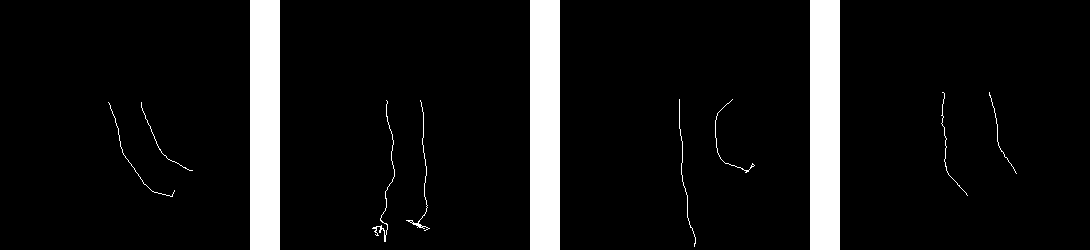
\includegraphics[width=0.8\textwidth]{2PersClusters.png}
    \end{center}
    \caption{Repräsentanten der größten Cluster mit zwei Personen.}
    \label{fig:2PersClusters}
\end{figure}
Zum einen handelt es sich um den Fall, dass zwei Personen durch den Aufnahmebereich laufen.
Dies ist die analoge Bewegung zum gefundenen Cluster bei drei Personen.
Der zweite Fall zeigt, wie sich zwei Personen dem Sensor nähern.
In Szenario drei bewegt sich eine Person zur Kamera,
während eine Andere lediglich durch das Bild läuft.
Im letzten Fall laufen zwei Personen gemeinsam zum oberen Bildrand.
Alle Szenarien werden durch das Tool gefunden.
Bei dieser großen Menge an Records fällt auf,
dass bei niedrigen Thresholds ähnliche Records teilweise noch in unterschiedlichen Clustern liegen
und erst in späteren Schritten kombiniert werden,
da andere Szenarien noch eine höhere Ähnlichkeit aufweisen.

Das Tool kann für Datensätze mit Ein- bis Zweitausend Records sehr effizient eingesetzt werden.
Auf einem heute typischen Heimrechner werden innerhalb weniger Minuten Ergebnisse geliefert.
Ab einigen Tausend Records nimmt die Bearbeitungszeit stark zu,
sodass unter Umständen mit mehreren Stunden Wartezeit zu rechnen ist.
Diese Limitierung sollte beachtet werden,
falls in Zukunft noch größere Datenmengen geclustert werden müssen.
Dann muss entweder ein leistungsfähigerer Rechner eingesetzt werden,
oder das Tool weiter optimiert werden.
Beispielweise kann über Parallelisierung nachgedacht werden.
Insgesamt befinden sich 3523 Records mit einer Person im gefilterten Datensatz.
Ab einer gewissen Menge treten allerdings kaum noch neue Bewegungsmuster auf.
Deshalb soll die Analyse im Folgenden auf eine Teilmenge mit 1000 beliebigen Records eingeschränkt werden.
Erneut wird überprüft, ob wiederkehrende Bewegungen korrekt erkannt werden.
\autoref{fig:1PersClusters} zeigt jeweils einen Repräsentanten der manuell erkannten Muster.
\begin{figure}[ht]
    \begin{center}
    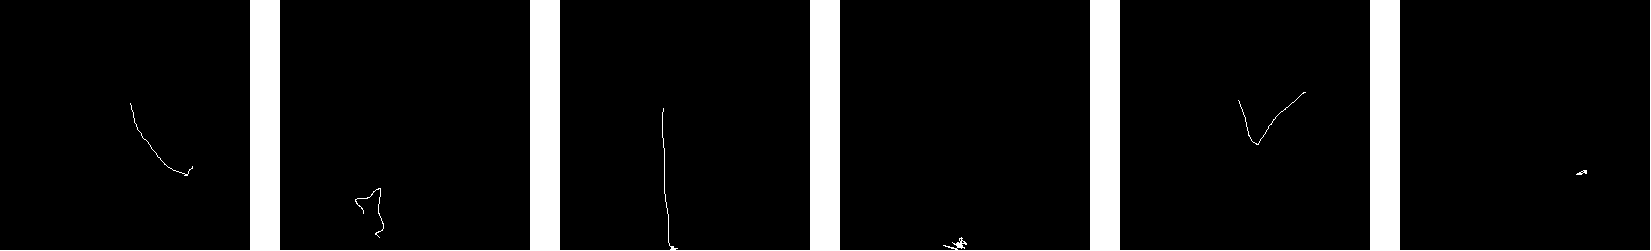
\includegraphics[width=\textwidth]{1PersClusters.png}
    \end{center}
    \caption{Repräsentanten der größten Cluster mit einer Person.}
    \label{fig:1PersClusters}
\end{figure}
Im ersten Fall bewegt sich eine Person durch den Aufnahmebereich,
während sie sich im zweiten Szenario unmittelbar vor der Kamera befindet.
Bild drei zeigt ein direktes Zugehen auf den Bildschirm.
Im vierten Fall und sechsten Fall steht die Person an verschiedenen Positionen beinahe still.
Szenario fünf zeigt, wie eine Person nach vorne läuft,
sich umdreht und wieder zurück läuft.
All diese Fälle können durch das Tool erkannt werden.
Zu erwähnen ist allerdings, dass manche Cluster bei hohen Thresholds bereits in andere Muster integriert werden.
So kann etwa das fünfte Szenario nur bei niedrigeren Thresholds erkannt werden,
während es bei höheren Werten unter Umständen bereits mit Cluster eins zusammengeführt wurde.
Dies verdeutlicht erneut, dass eine sinnvolle Suche nach Clustern möglich ist,
diese aber dennoch manuell betrachtet werden müssen.
Dabei sollte auch mit verschiedenen Thresholds experimentiert werden.

Die Auswertung des gesamten Datensatzes bestätigt also was die Minimalbeispiele bereits vermuten liesen.
Das Tool kann erfolgreich genutzt werden, um sinnvolle Cluster auf den Kinect-Bewegungsdaten zu finden.
Im Folgenden Abschnitt soll abschließend die Güte der gefundenen Cluster an einigen Beispielen
überprüft werden.

\section{Statistische Analyse}
\label{6-Statistical}
Abschließend soll mithilfe von \emph{deskriptiven Statistiken} überprüft werden,
ob ein Zusammenhang zwischen den Record-Bestandteilen eines Clusters besteht.
Der Grad der Übereinstimmung liefert Informationen zur Ähnlichkeit.
Konkret werden nun für die Komponenten einiger gefundener Cluster
die Standardabweichung, der Mittelwert, das Maximum und das Minimum für die x-Laufwege berechnet
und tabellarisch dargestellt werden.
Dazu werden teilweise die Minimalbeispiele aus \autoref{6-GroundTruth} wieder aufgegriffen.
Als erstes werden die Werte für drei beliebige Records des ersten Cluster mit drei Personen berechnet (\autoref{fig:Clusters}).
Sie werden in \autoref{tbl:ClustThreePers} dargestellt.
Die Ergebnisse sind auf zwei Nachkommastellen gerundet.
\begin{center}
    \begin{table}[ht]
    \begin{tabular}{ |c|c|c|c|c| } 
     \hline
     Record & Mittelwert & Standardabw. & Minimum & Maximum \\
     \hline \hline
     2017-04-05 08.16.53.128 +02.00
     & -0,79
     & 0,50
     & -1,79
     & 0,17
     \\
     \hline
     2017-04-05 10.56.51.141 +02.00
     & -0,73
     & 0,63
     & -2,20
     & 0,41
     \\
     \hline
     2017-04-05 12.29.05.007 +02.00
     & -0,66
     & 0,64
     & -1,96
     & 0,44
     \\
     \hline
    \end{tabular}
    \caption{Deskriptive Statistiken für das Cluster mit drei Pers.}
    \label{tbl:ClustThreePers}
    \end{table}
  \end{center}
  Alle Mittelwerte und Standardabweichungen bewegen sich in einem ähnlichen Rahmen.
  Dadurch wird bestätigt, dass die Records einen inhaltlichen Zusammenhang aufweisen.
  Ähnliches ist beim ersten Cluster mit zwei Personen aus \autoref{fig:Clusters} zu erkennen.
  Auch hier ähneln sich die Werte, wie in \autoref{tbl:ClustTwoPers} zu sehen ist.
  \begin{center}
    \begin{table}[ht]
    \begin{tabular}{ |c|c|c|c|c| } 
     \hline
     Record & Mittelwert & Standardabw. & Minimum & Maximum \\
     \hline \hline
     2017-04-05 08.16.53.128 +02.00
     & -0,88
     & 0,48
     & -1,77
     & -0,03
     \\
     \hline
     2017-04-05 10.56.51.141 +02.00
     & -0,68
     & 0,58
     & -1,77
     & 0,31
     \\
     \hline
     2017-04-05 12.29.05.007 +02.00
     & -0,80
     & 0,55
     & -1,85
     & 0,16
     \\
     \hline
    \end{tabular}
    \caption{Deskriptive Statistiken für das Cluster mit zwei Pers.}
    \label{tbl:ClustTwoPers}
    \end{table}
  \end{center}
  Setzt man in diesem Beispiel allerdings den Threshold noch höher,
  sodass die gefundenen Cluster augenscheinlich nicht mehr sinnvoll erscheinen
  erhält man die Werte in \autoref{tbl:ClustTwoPersHighThreshold}.
  \begin{center}
    \begin{table}[ht]
    \begin{tabular}{ |c|c|c|c|c| } 
     \hline
     Record & Mittelwert & Standardabw. & Minimum & Maximum \\
     \hline \hline
     2017-04-05 08.16.53.128 +02.00
     & -0,61
     & 0,61
     & -1,67
     & 0,45
     \\
     \hline
     2017-04-05 10.56.51.141 +02.00
     & -0,53
     & 0,36
     & -1,08
     & -0,14
     \\
     \hline
     2017-04-05 12.29.05.007 +02.00
     & -0,14
     & 0,54
     & -1,23
     & 1,07
     \\
     \hline
    \end{tabular}
    \caption{Deskriptive Statistiken für das Cluster mit zwei Pers. (hoher Threshold).}
    \label{tbl:ClustTwoPersHighThreshold}
    \end{table}
  \end{center}
  Hier sind größere Differenzen erkennbar.
  Dies betont einerseits erneut die bedeutende Rolle eines geeigneten Thresholds
  und andererseits, dass die Bestimmung der Güte mittels desktiptiver Statistiken möglich ist.
  Die Records der Cluster der beiden ersten Beispiele weisen tatsächlich eine hohe Ähnlichkeit auf.